\documentclass{article}
\usepackage[margin=1in,a4paper]{geometry}
\usepackage[utf8]{inputenc}
\usepackage[cyr]{aeguill}
\usepackage[francais]{babel}
\usepackage{hyperref}
\usepackage{amsmath}
\usepackage{gensymb}
\usepackage{enumitem,amssymb}
\newlist{checks}{itemize}{2}
\setlist[checks]{label=$\square$}
\usepackage{graphicx}
\usepackage{amsthm}
\usepackage{amsfonts}
\usepackage{multicol}
\usepackage{pgfplots}
\pgfplotsset{compat=newest}
\usetikzlibrary{calc}
\usepackage{mathtools}
\usepackage{array}
\usepackage[T1]{fontenc}
\usepackage{lmodern}
\usepackage{tabularx}
\usepackage{fancyhdr}
\usepackage{pst-func}
\usepackage{xcolor}
\usepackage{nicefrac}
\usepackage{mdframed}
\usepackage[boxed,vlined]{algorithm2e}
\usepackage{cleveref}
\newcommand{\Lim}[1]{\raisebox{0.5ex}{\scalebox{1}{$\displaystyle \lim_{#1}\;$}}}
\usepackage{float}
%\usepackage[top=2.5cm, bottom=2cm, left=2cm, right=2cm, showframe]{geometry}
\usepackage[top=2.5cm, bottom=2cm, left=2cm, right=2cm]{geometry}
\newcommand{\N}{\mathbb{N}}
\newcommand{\R}{\mathbb{R}}
\renewcommand{\C}{\mathbb{C}}
\renewcommand{\P}{\mathbb{P}}
\newcommand{\w}{\omega}
\newcommand{\p}{\partial}
\newcommand{\cross}{\times}
\newcommand{\Col}{\text{Col}}
\newcommand{\Tr}{\text{Tr}}
\newcommand{\bigzero}{\makebox(0,0){\text{\huge0}}}
\DeclareMathOperator{\Ima}{Im}
\DeclareMathOperator{\Vect}{Vect}
\usepackage{mathtools, stmaryrd}
\usepackage{xparse} \DeclarePairedDelimiterX{\Iintv}[1]{\llbracket}{\rrbracket}{\iintvargs{#1}}
\NewDocumentCommand{\iintvargs}{>{\SplitArgument{1}{,}}m}
{\iintvargsaux#1} %
\NewDocumentCommand{\iintvargsaux}{mm} {#1\mkern1.5mu..\mkern1.5mu#2}
\newcommand{\Cc}{{\mathbb{C}}}
\newcommand{\Ct}{\Cc^\times}
\newcommand{\Hh}{{\mathbb{H}}}
\newcommand{\Nn}{{\mathbb{N}}}
\newcommand{\Zz}{{\mathbb{Z}}}
\newcommand{\Zzn}{\Zz/n\Zz}
\newcommand{\ZzNt}{(\Zz/N\Zz)^\times}%quotient 
\newcommand{\Rr}{{\mathbb{R}}}
\newcommand{\Rt}{{\Rr^\times}}
\newcommand{\Qt}{{\Qq^\times}}
\newcommand{\Qq}{{\mathbb{Q}}}
% Custom titling
\usepackage{titling}
\usepackage{tcolorbox}

\title{\textbf{Analyse Avancée -- Série 2}}

\renewcommand{\maketitlehookb}{
\begin{center}

\includegraphics[width=2cm]{Cours/assets/imgs/logo-round.png}
\end{center}
}

\author{Students 4 Students}
\date{Septembre 2022}

% Exercises environment and styling
\usepackage{amsthm}
\newtheoremstyle{exercice}%
    {3pt}% Space above
    {3pt}% Space below
    {\large}% Body font
    {}% Indent amount
    {\bfseries}% Theorem head font
    {}% Punctuation after theorem heading
    {\newline}% Space after theorem heading
    {\thmname{#1}\thmnumber{ #2}\thmnote{: #3}}% Theorem head spec (can be left empty, meaning ‘normal’)
\theoremstyle{exercice}
\newtheorem{exercice}{Exercice}


\begin{document}

% Header
\pagestyle{fancy}
\fancyhead[L]{Students 4 Students}
\fancyhead[C]{\textit{Analyse avancée - Série 2}}
\fancyhead[R]{Septembre 2022}

\maketitle


\begin{exercice}[Limites usuelles]
    
Dans la pratique, nous utilisons des compositions de limites usuelles pour calculer les limites des suites rapidement. Il faut donc les démontrer, comme tout en mathématiques! Trouver les limites à l'infini des suites suivantes :

\begin{enumerate}
    

    \begin{multicols}{2}
    \item $x_n=n$
    \item $x_n= n^p$, $p>0$
    \item $x_n=n^p$, $p\leq 0$
    \item $x_n= a \cdot n^p$, $a,p\in \Rr$
    \item $x_n= \dfrac{n^p}{n^q}$, $p,q\in \Rr$
    \item $x_n=\dfrac{a_pn^p+a_{p-1}n^{p-1}+...+a_0}{b_qn^q+b_{q-1}n^{q-1}+...+b_0}$, $a_i,b_i\in \Rr$, $a_p$ et $b_q$ non nuls et $p,q \in \Rr ^+$
    \end{multicols}
\end{enumerate}
\end{exercice}
% \section{Limites usuelles avancées}
% Ces limites sont plus ardus à démontrer et nécessite des notions qui ne sont pas enseignées dans ce cours. Donc, cet exercice est facultatif. 
% Montrer les limites suivantes
% \begin{enumerate}
%         \item $\underset{{n\to \infty}}\lim \dfrac{x^n}{n!}$, avec $n!=n\cdot (n-1)\cdot \cdot \cdot 3\cdot 2\cdot 1$
%         \item $\underset{{n\to \infty}}\lim \left(1+\dfrac{1}{n}\right)^k$=1, $k\in \Nn$ fixé
% \end{enumerate}
\newpage
\begin{exercice}[Sous-suites, Principe des deux gendarmes]
\\ \newline
\textbf{Sous-suites}
Commençons par étudier la convergence de la suite suivante:
\begin{equation}
    x_n = \sin(\frac{n \pi}{2}) \quad \forall n\in \Nn
\end{equation}

\textbf{a)} Représentez quelques points de la suite sur la Figure \ref{fig:exo2.1a}.\\

\begin{figure}[H]
    \centering
    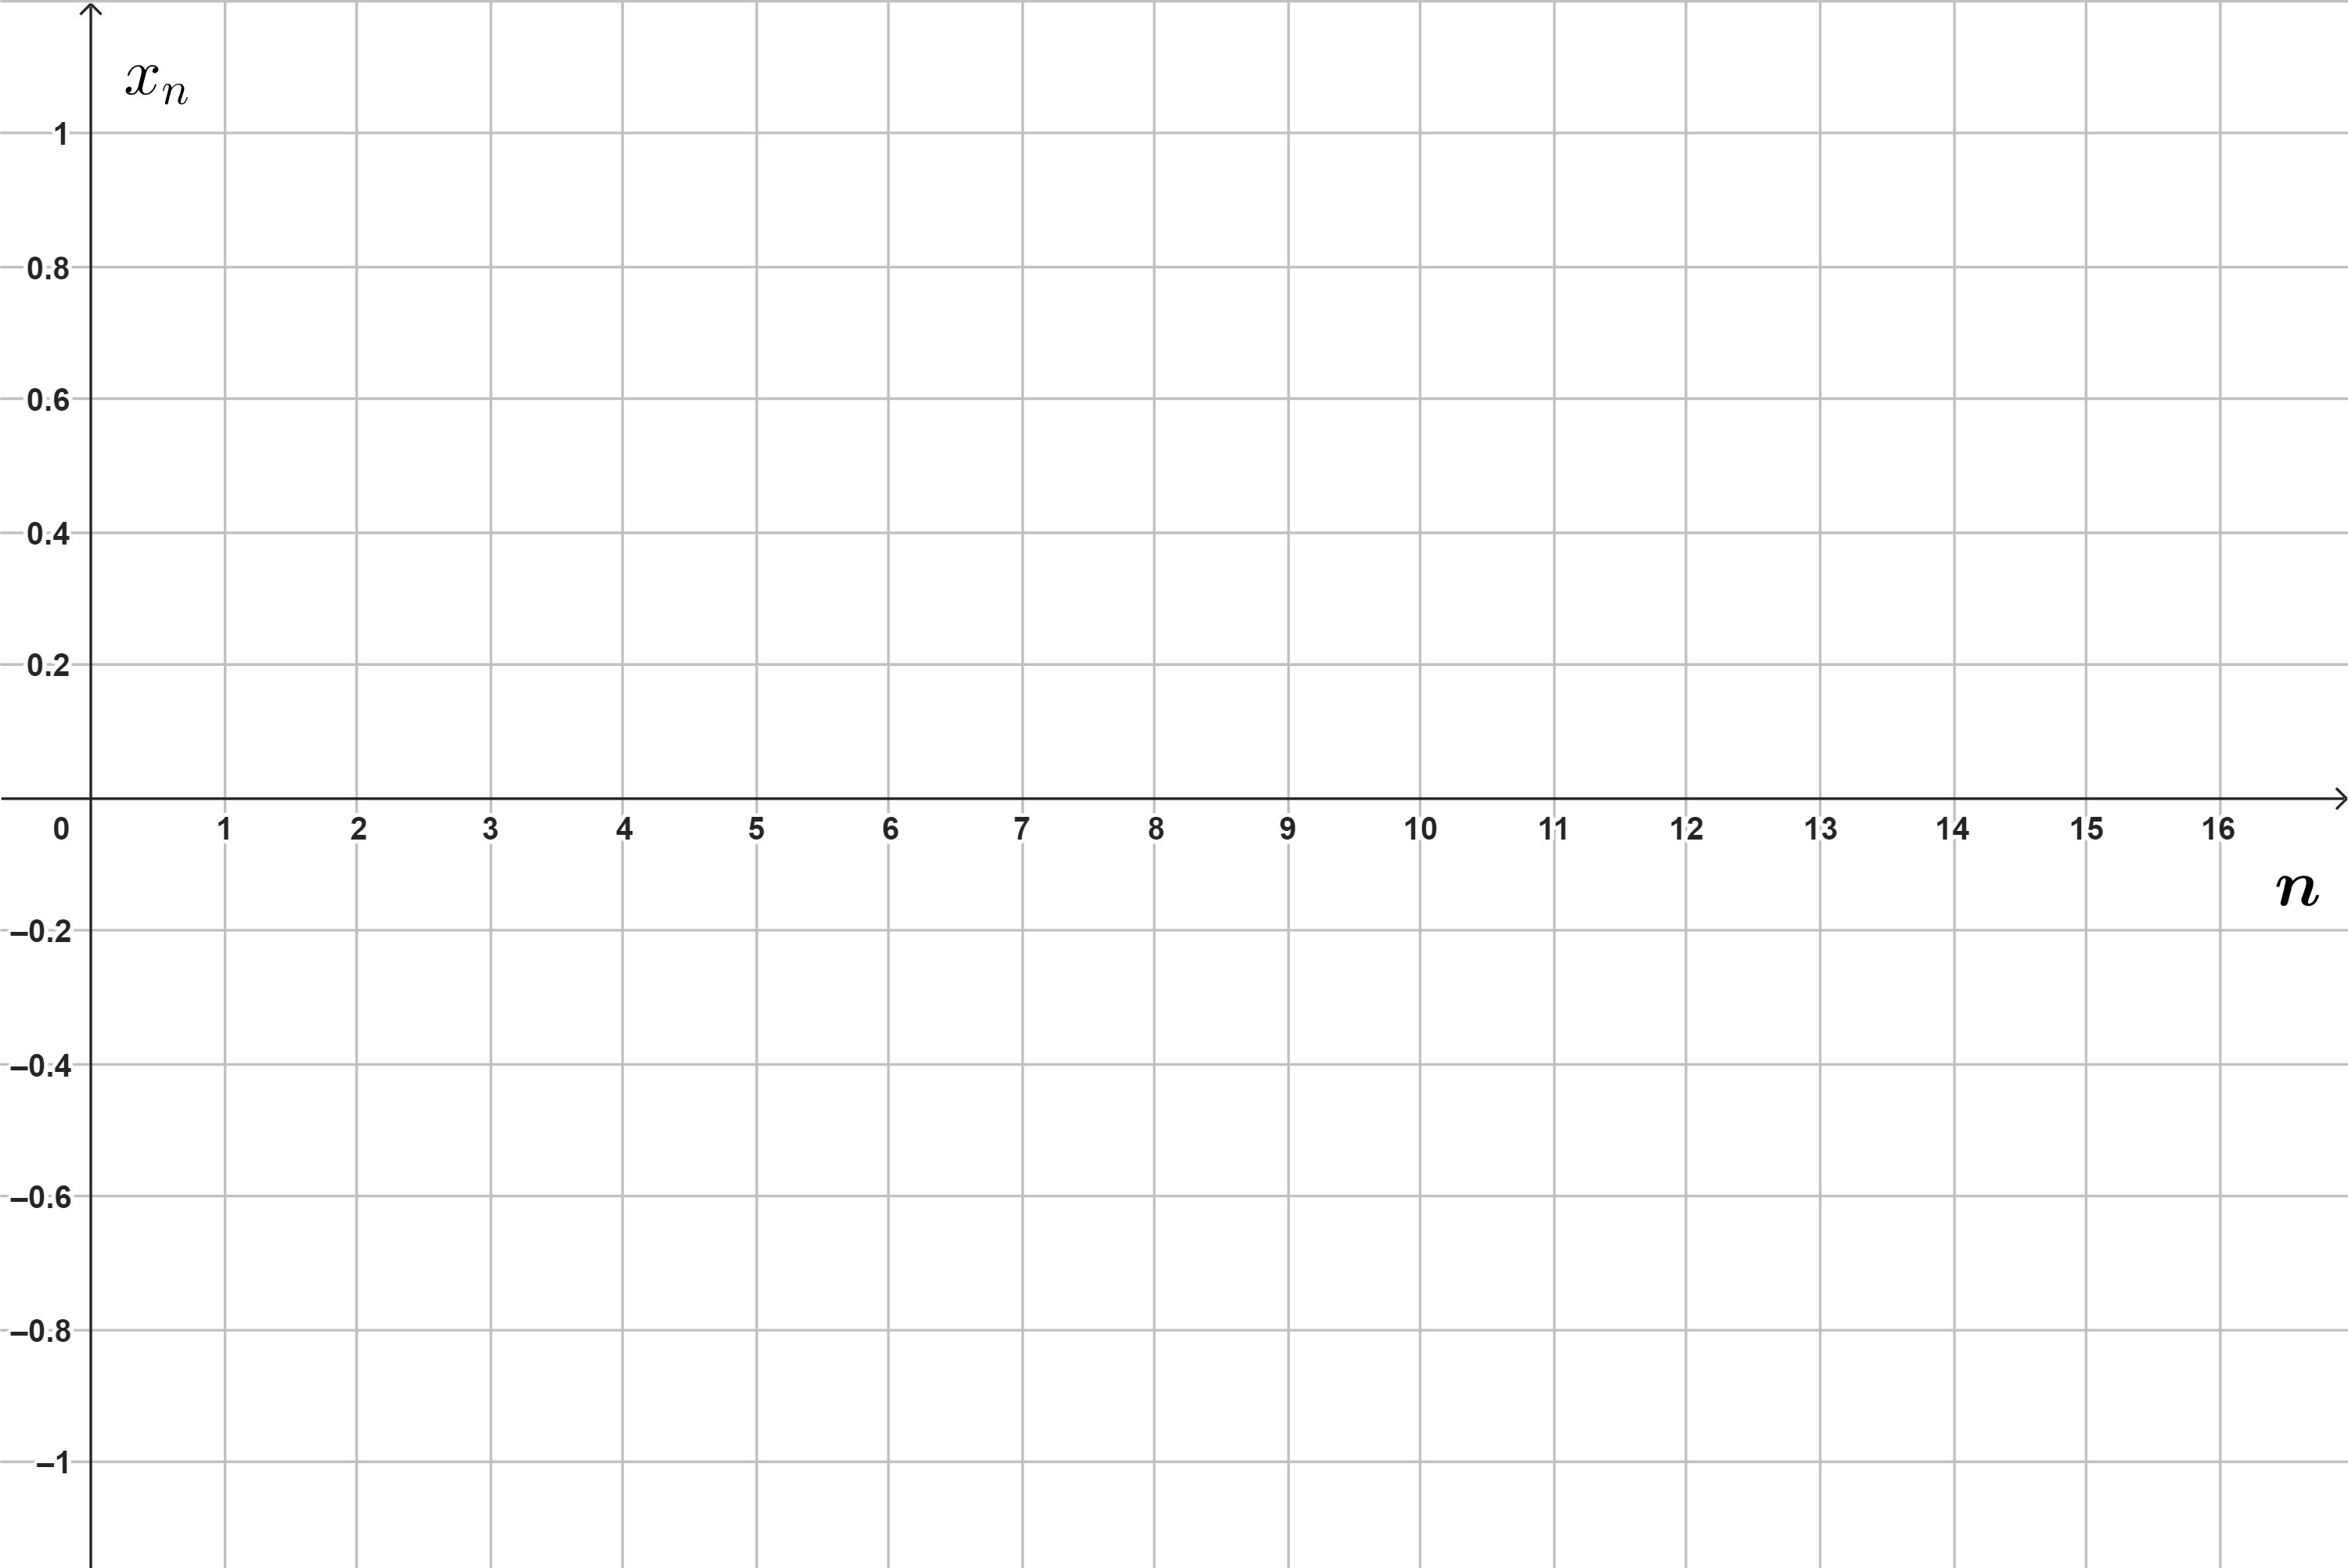
\includegraphics[scale=0.8]{Exercices/exo_sabri.png}
    \caption{Exercice \textbf{2.1 a)}}
    \label{fig:exo2.1a}
\end{figure}

\textbf{b)} Cette suite converge-t-elle? Sinon, pouvez-vous donner une sous-suite qui converge? \\
\textbf{Notez:} Le théorème de Bolzano-Weierstrass nous dit que toute suite bornée admet une sous-suite convergente (elle n'est pas toujours facile à trouver cependant). \\

\textbf{c)} Quelles sont les limites inférieure et supérieure de $x_n$ ? \\

Passons à présent à la suite suivante:
\begin{equation}
    y_n = \frac{1}{n} \sin(\frac{n \pi}{2}) \quad \forall n\in \Nn_0
    \label{exo_sous_suite}
\end{equation}

\textbf{d)} Représentez quelques points de cette suite sur la Figure \ref{fig:exo2.1d}. Cette suite converge-t-elle? Sinon, pouvez-vous donner une sous-suite qui converge? \\

\begin{figure}[H]
    \centering
    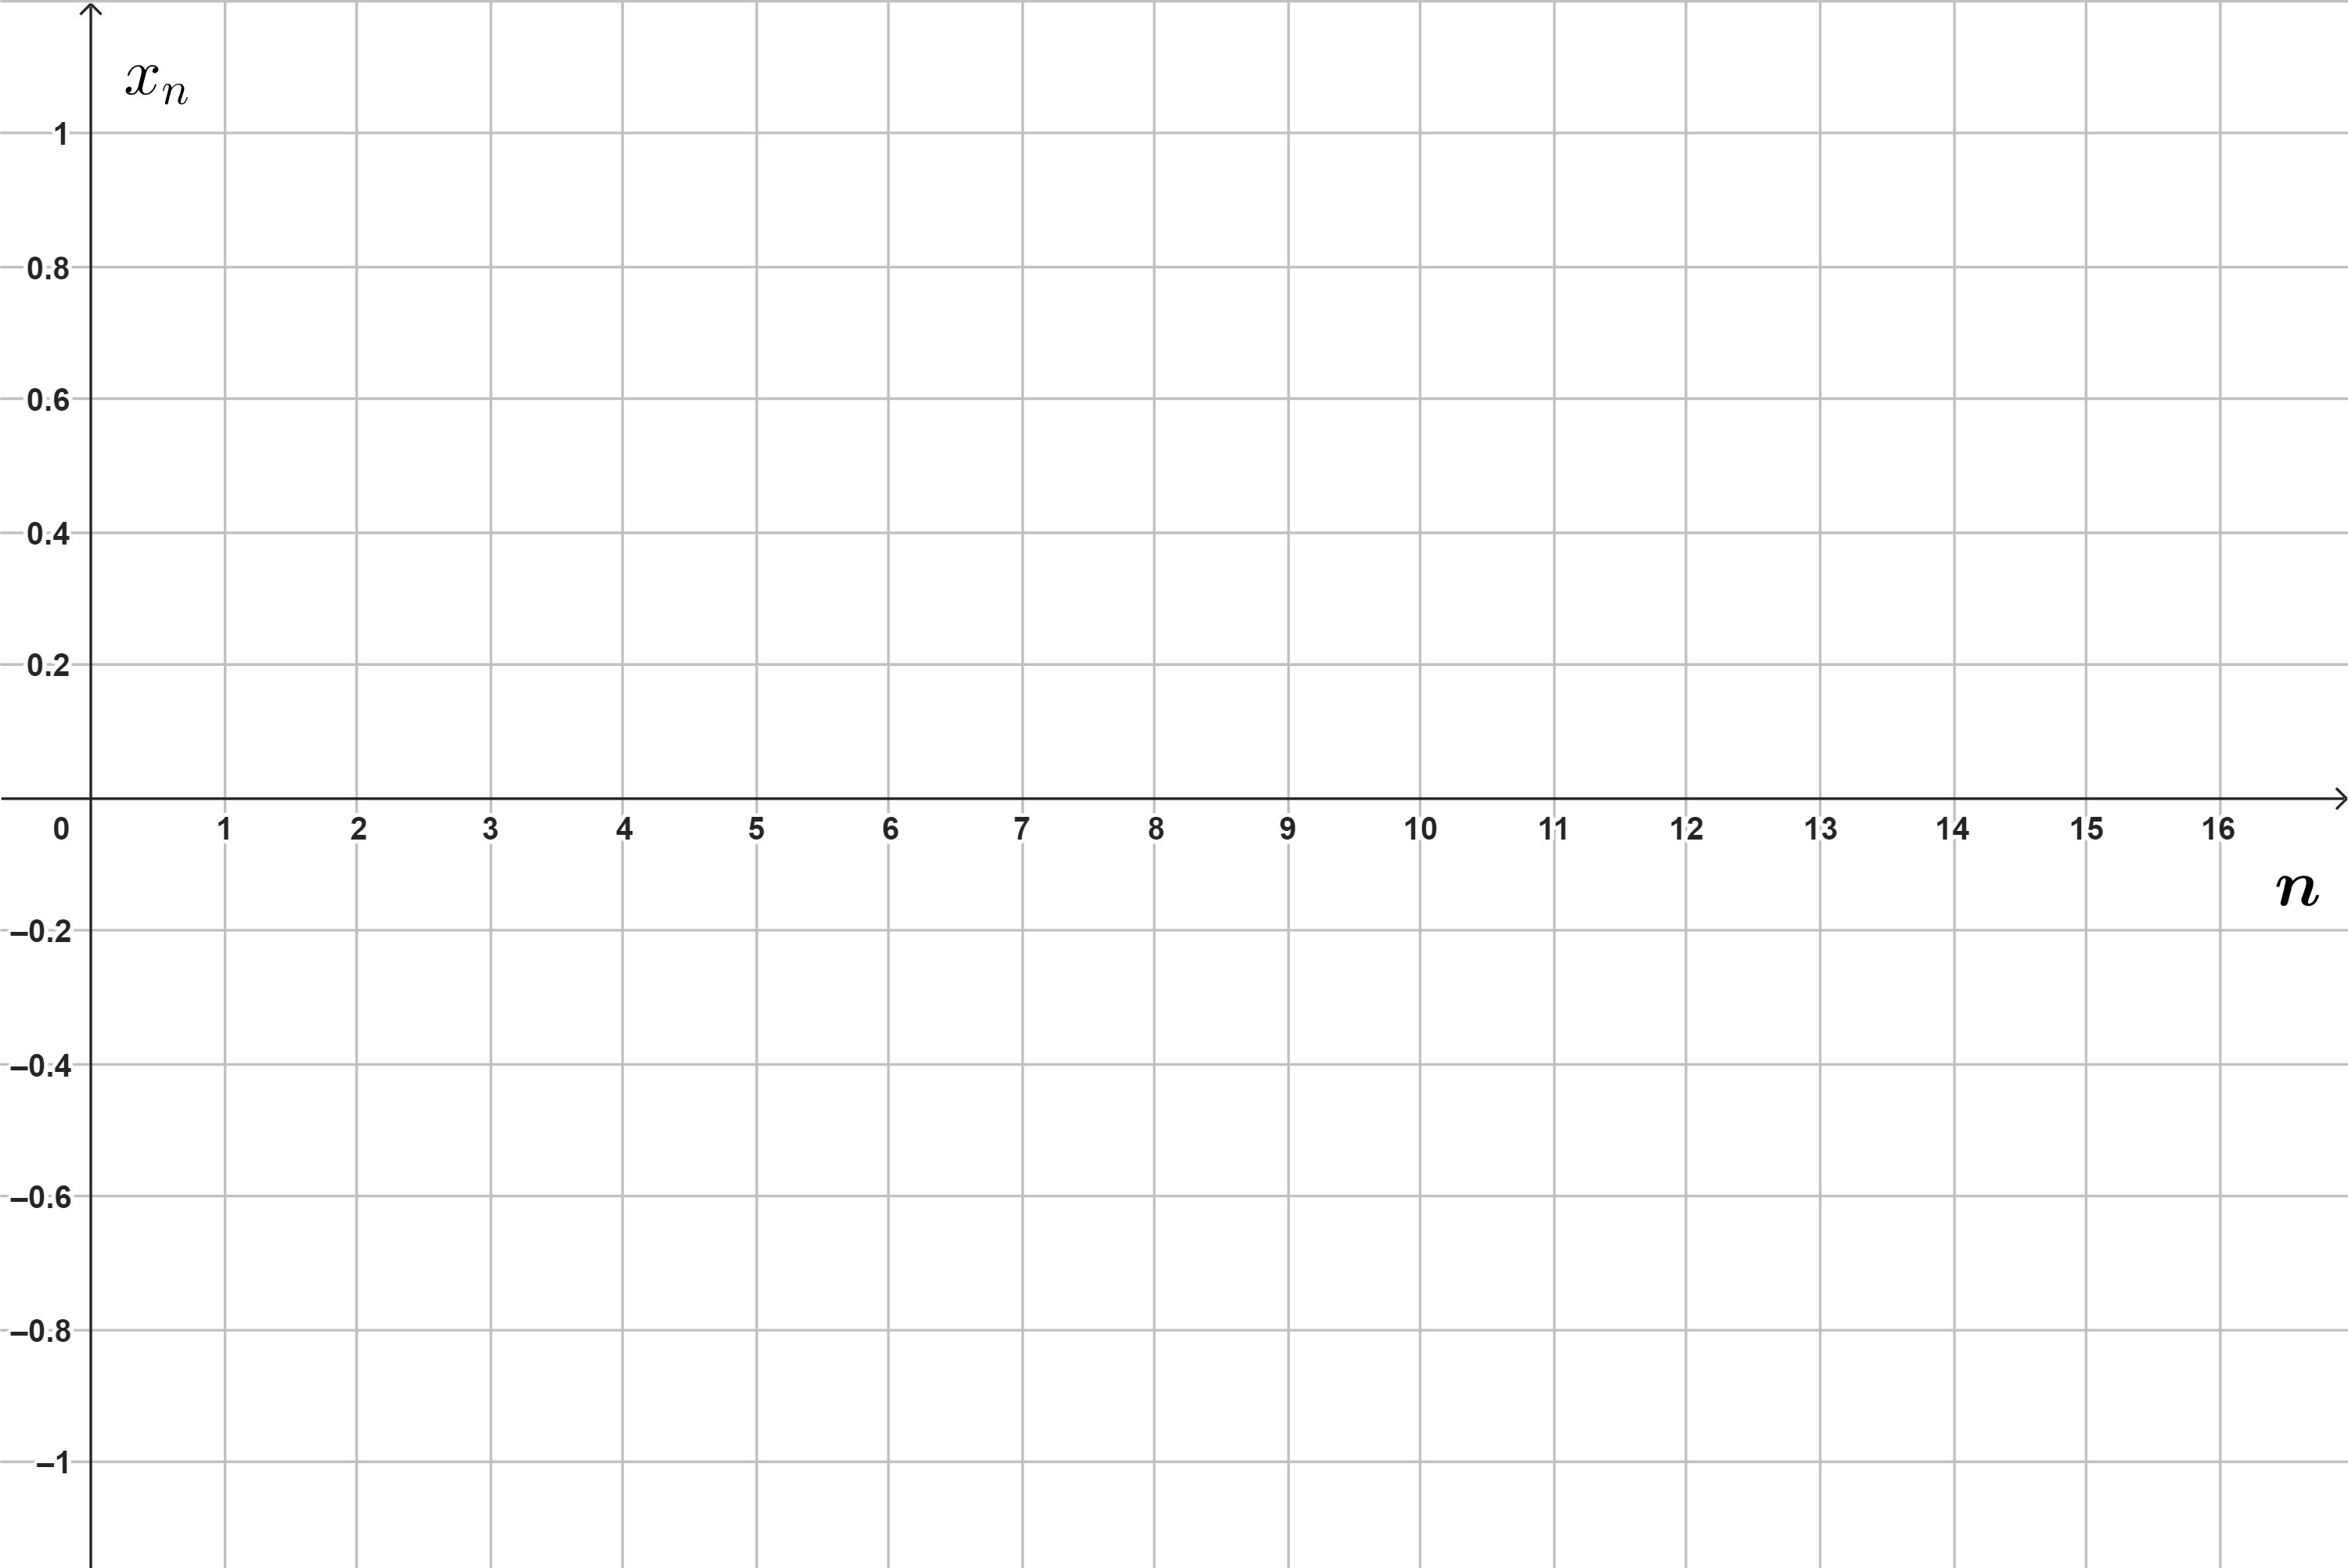
\includegraphics[scale=0.8]{Exercices/exo_sabri.png}
    \caption{Exercice \textbf{2.1 d)}}
    \label{fig:exo2.1d}
\end{figure}\\ \\

\textbf{e)} La sous-suite d'une suite convergente peut-elle converger vers une valeur différente? Si oui, donner un exemple. Sinon, démontrez-le.\\ \newline

\textbf{Principe des deux gendarmes}
En traçant quelques points de la suite \eqref{exo_sous_suite}, on voit clairement qu'elle converge. Montrons-le plus rigoureusement en utilisant le Principe des deux gendarmes.\\

\textbf{a)} Trouvez deux suites $(v_n)$ et $(w_n)$ qui convergent vers $0$ et telles que $v_n \leq y_n \leq w_n$. Tracez-les sur la Figure \ref{fig:exo2.1d} afin de vous assurer que les deux gendarmes font bien leur travail. \\

\textbf{b)} Démontrez que la convergence de $(v_n)$ et $(w_n)$ implique celle de $(y_n)$ (en d'autres mots, démontrez le Principe des deux gendarmes, bien sûr sans regarder le polycopié ou vos notes...). \\

\faLightbulbO \quad \fbox{\textbf{Discutez}} Quels ``gendarmes" utiliseriez-vous pour la suite suivante ?
\begin{equation}
    z_n = \frac{1}{n+\sin(n)}, \quad n \geq 2
\end{equation}
\end{exercice}
\begin{exercice}[Suite de Cauchy]
Toute suite réelle converge si et seulement si c'est une suite de Cauchy. Nous allons essayer de mieux comprendre ce qu'est une suite de Cauchy en étudiant l'exemple suivant:
\begin{equation}
    x_n = \frac{(-1)^n}{n} \quad \forall n\in \Nn_0
\end{equation}

\textbf{a)} Montrez que la suite $(x_n)$ est de Cauchy en utilisant la définition. Aidez-vous de la Figure \ref{fig:exo3a} pour mieux visualiser le problème si nécessaire.\\

\begin{figure}[H]
    \centering
    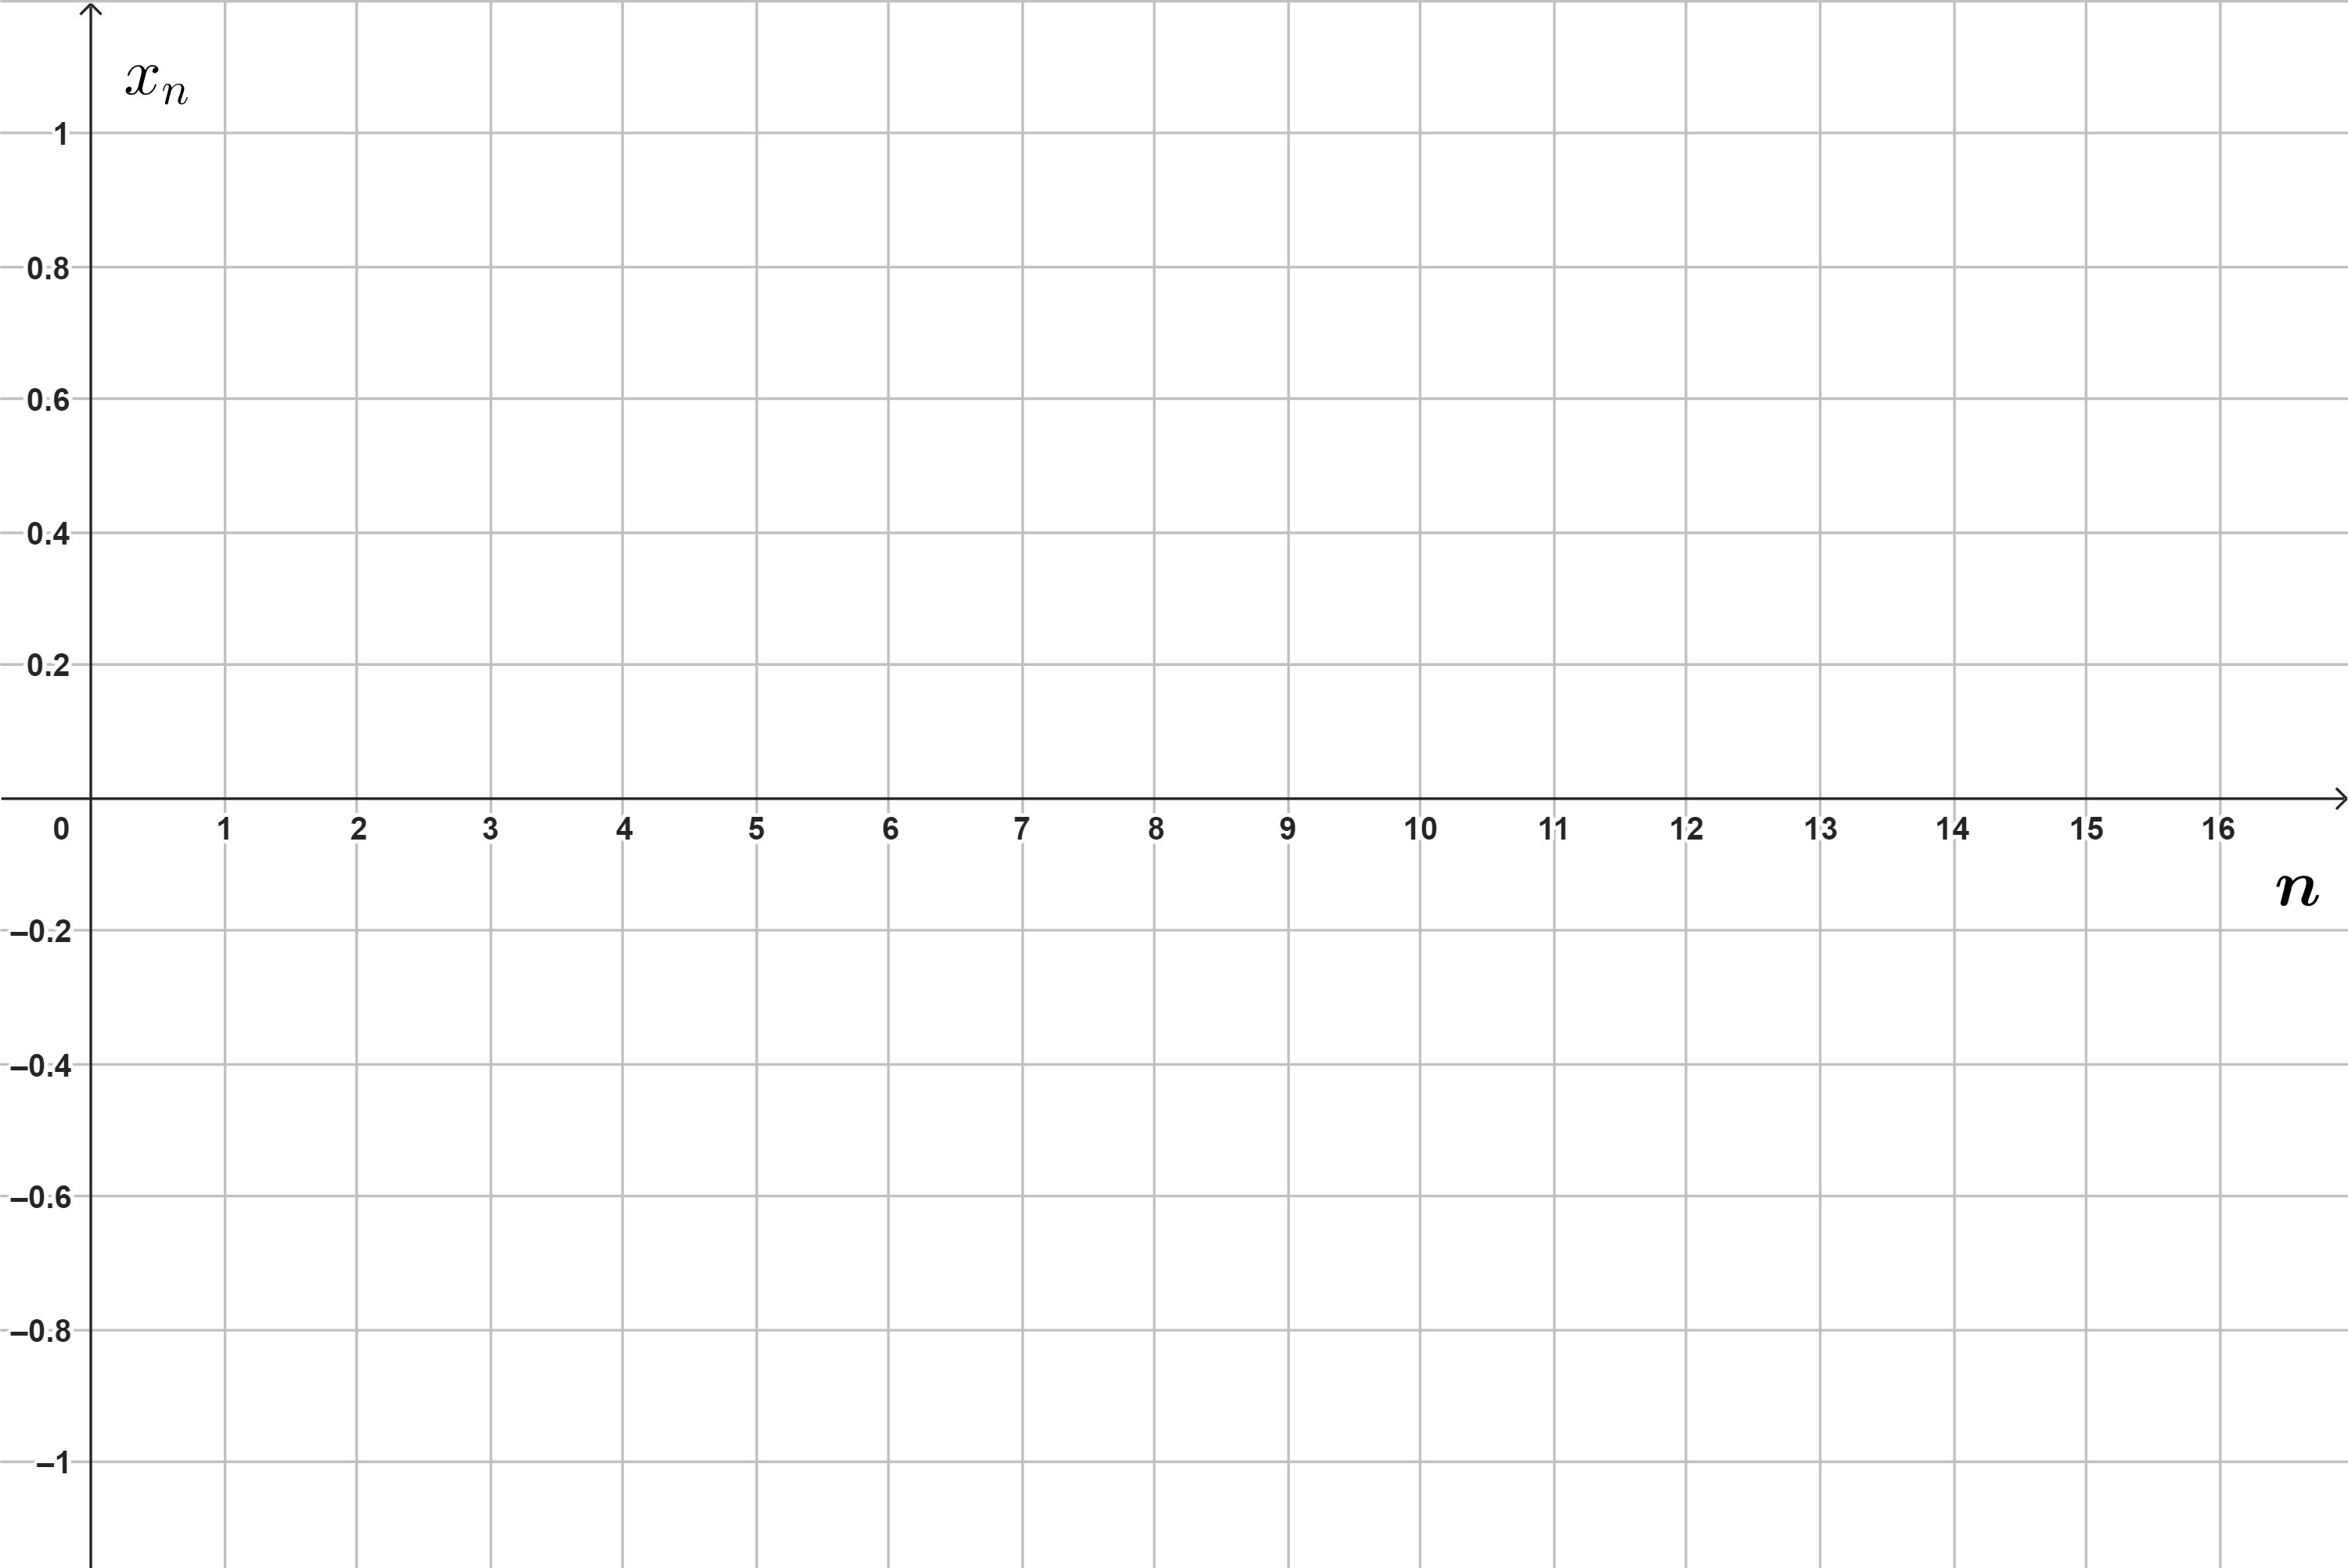
\includegraphics[scale=0.8]{Exercices/exo_sabri.png}
    \caption{Exercice \textbf{3 a)}}
    \label{fig:exo3a}
\end{figure}\\ \\

\textbf{b)} Montrez par contradiction qu'une suite de Cauchy est bornée. \\
 \\

\faLightbulbO \quad \fbox{\textbf{Discutez}} A l'exercice \textbf{b)}, aurait-on pu démontrer la proposition en partant du principe que la suite n'est pas de Cauchy, pour ensuite montrer que cela contredit la suite bornée? \\


    
\end{exercice}

\begin{exercice}
Montrer en utilisant la définition de limite que \[\lim_{n\to\infty}\cos{\frac{2\pi n^{3}+2}{n^{2}}} = 1.\] \\ \\
\noindent
\textit{Indication :} On a pour tout $a, b \in \R$, \[\cos a - \cos b = -2\sin{\frac{a+b}{2}}\,\sin{\frac{a-b}{2}}\] 

    
\end{exercice}

\begin{exercice}
    Calculer la limite suivante en utilisant la périodicité du sinus:

    \begin{equation}
        \lim_{n\to \infty} \sin(\pi \sqrt{4 n^2+n}) 
    \end{equation}
       
\end{exercice}
\end{document}